\documentclass[12pt,oneside]{uhthesis}
\usepackage{subfigure}
\usepackage[ruled,lined,linesnumbered,titlenumbered,algochapter,spanish,onelanguage]{algorithm2e}
\usepackage{amsmath}
\usepackage{amssymb}
\usepackage{amsbsy}
\usepackage{caption,booktabs}
\captionsetup{ justification = centering }
%\usepackage{mathpazo}
\usepackage{float}
\setlength{\marginparwidth}{2cm}
\usepackage{todonotes}
\usepackage{listings}
\usepackage{xcolor}
\usepackage{multicol}
\usepackage{graphicx}
\floatstyle{plaintop}
\restylefloat{table}
\addbibresource{Bibliography.bib}
% \setlength{\parskip}{\baselineskip}%
\renewcommand{\tablename}{Tabla}
\renewcommand{\listalgorithmcfname}{Índice de Algoritmos}
%\dontprintsemicolon
\SetAlgoNoEnd

\definecolor{codegreen}{rgb}{0,0.6,0}
\definecolor{codegray}{rgb}{0.5,0.5,0.5}
\definecolor{codepurple}{rgb}{0.58,0,0.82}
\definecolor{backcolour}{rgb}{0.95,0.95,0.92}

\lstdefinestyle{mystyle}{
    backgroundcolor=\color{backcolour},   
    commentstyle=\color{codegreen},
    keywordstyle=\color{purple},
    numberstyle=\tiny\color{codegray},
    stringstyle=\color{codepurple},
    basicstyle=\ttfamily\footnotesize,
    breakatwhitespace=false,         
    breaklines=true,                 
    captionpos=b,                    
    keepspaces=true,                 
    numbers=left,                    
    numbersep=5pt,                  
    showspaces=false,                
    showstringspaces=false,
    showtabs=false,                  
    tabsize=4
}

\lstset{style=mystyle}

\title{AutoGOAL model-based}
\author{\\\vspace{0.25cm}Karel Díaz Vergara}
\advisor{\\\vspace{0.25cm}Carlos Bermudez Porto\\\vspace{0.2cm}Alejandro Piad Morffis}
\degree{Licenciado en (Matemática o Ciencia de la Computación)}
\faculty{Facultad de Matemática y Computación}
\date{Fecha\\\vspace{0.25cm}\href{https://github.com/Karelito00/thesis}{github.com/Karelito00/thesis}}
\logo{Graphics/uhlogo}
\makenomenclature

\renewcommand{\vec}[1]{\boldsymbol{#1}}
\newcommand{\diff}[1]{\ensuremath{\mathrm{d}#1}}
\newcommand{\me}[1]{\mathrm{e}^{#1}}
\newcommand{\pf}{\mathfrak{p}}
\newcommand{\qf}{\mathfrak{q}}
%\newcommand{\kf}{\mathfrak{k}}
\newcommand{\kt}{\mathtt{k}}
\newcommand{\mf}{\mathfrak{m}}
\newcommand{\hf}{\mathfrak{h}}
\newcommand{\fac}{\mathrm{fac}}
\newcommand{\maxx}[1]{\max\left\{ #1 \right\} }
\newcommand{\minn}[1]{\min\left\{ #1 \right\} }
\newcommand{\lldpcf}{1.25}
\newcommand{\nnorm}[1]{\left\lvert #1 \right\rvert }
\renewcommand{\lstlistingname}{Ejemplo de código}
\renewcommand{\lstlistlistingname}{Ejemplos de código}

\begin{document}

\frontmatter
\maketitle

\begin{dedication}

\end{dedication}
\begin{acknowledgements}
Quiero agradecer a mi mamá que me apoyó durante toda la carrera incluso estando lejos, por tanto tiempo, siempre me ayudó y me escuchó. A mi papá que no ha dejado de preocuparse un día tanto por mi desempeño como por mi salud. A mi hermana Karina que ha sido la compañera con la que he disfrutado tantos bellos momentos. A mi hermano Jorgito que gracias a él muchas veces he tomado las decisiones correctas y me ha sabido guiar.

A mi amigo Samuel con el cual llevo compartiendo desde los inicios y siempre me ha extendido su mano sin importar lo que conlleve, a su novia Arlen que me ha tratado como uno más de la familia.
A Damián, Lily, Elizabeth, Aitana, Enmanuel, Gabriel, Lopetegui, Mauricio y Rodovaldo por los momentos y las risas que hemos compartido(se me quedan muchos más).
Quiero también agradecer a todos los que formaron parte de mi vida en beca y que de alguna forma dentro de las dificultados hicieron que fuera divertido.
A Eziel que siempre tiene buenas películas para ver.
A mi amigo Frank Abel por las tantas noches que pasamos compartiendo el desarrollo de proyectos.
A Alben, el cual considero una persona genial, que más que un amigo es un hermano que me ha acompañado tanto en los buenos momentos como en los malos.
A mi tutor Carlos Bermudez que fue paciente conmigo y siempre estuvo ahí para resolver mis dudas.
A Piad y Suilan que han sido unos profesores increíbles en los cuales siempre he encontrado inspiración.
A mis profesores, amigos y aquellas personas las cuales de alguna forma u otra aportaron su granito a lo que soy hoy, gracias.
\end{acknowledgements}
\begin{opinion}
En la actualidad el Aprendizaje Automático ha llegado a todas las ramas de la industria, ayudando a resolver un gran número de problemas pero creando la necesidad de un enorme número de expertos para poder utilizar las herramientas adecuadas en cada caso.
En este escenario el AutoML propone una solución ayudando con la selección de forma automática de las mejores soluciones con el problema añadido de que incrementa el costo computacional ya que tiene que evaluar muchas soluciones para resolver cada problema. El área de investigación en que incursiona el estudiante está relacionada con la inclusión de modelos preentrenados a un sistema de AutoML heterogéneo.

El estudiante Karel Díaz Vergara en esta investigación se adentra en un tema del estado del arte de gran actualidad y para eso tuvo que utilizar conocimientos de varias asignaturas de la carrera y otros que no son parte del currículum estándar. Su propuesta implicó estudiar el estado del arte de las herramientas de AutoML, así como las arquitecturas de modelos preentrenados más usadas en este dominio. Además, realizó una implementación computacional de varias de estas arquitecturas, de forma que son compatibles con AutoGOAL, una biblioteca de AutoML del estado del arte.

Sus resultados, aunque modestos debido al alto costo computacional de entrenar dichas arquitecturas, resultan convincentes, pues permiten atacar algunos tipos de problemas que hasta ahora no eran solubles en AutoGOAL eficientemente. Además, la implementación es fácilmente extensible a nuevos modelos preentrenados que puedan ser aplicados en tareas novedosas.

Para poder afrontar el trabajo, el estudiante tuvo que revisar literatura científica relacionada con la temática así como soluciones existentes y bibliotecas de software que pueden ser apropiadas para su utilización. Todo ello con sentido crítico, determinando las mejores aproximaciones y también las dificultades que presentan. Todo el trabajo fue realizado por el estudiante con una elevada constancia, capacidad de trabajo y habilidades, tanto de gestión, como de desarrollo y de investigación.

Por estas razones pedimos que le sea otorgada al estudiante Karel Díaz Vergara la máxima calificación y, de esta manera, pueda obtener el título de Licenciado en Ciencia de la Computación.

\begingroup
  \centering
  \wildcard{Dr. Alejandro Piad Morffis}
  \hspace{1cm}
  \wildcard{Lic. Carlos Bermudez Porto}
  \par
\endgroup

\end{opinion}
\begin{resumen}
	La inteligencia artificial a lo largo de los años se ha vuelto crucial en la resolución de problemas en diferentes áreas. Numerosos avances se han logrado en el campo de visión por computadora o en el procesamiento del lenguaje natural. Incluso las grandes industrias han estado desarrollando servicios que muchas veces tienen como objetivo entregar modelos de calidad a los usuarios y abstraerlos de la parte científica. A día de hoy ha surgido una comunidad que se ha encargado de crear métodos que combinan diferentes algoritmos de machine learning y diferentes configuraciones de estos generando espacios de búsquedas los cuales son explorados de manera inteligente para encontrar la mejor solución a un problema. Estos métodos pertenecen al área llamada Auto Machine Learning. El AutoML es el proceso de automatizar la resolución de problemas de machine learning en sus diferentes etapas, como el preproceso y limpieza de los datos, la selección de features, selección del conjunto de algoritmos a utilizar, la configuración de los parámetros, la optimización de estos procesos, entre otros, con el objetivo de que se reduzca considerablemente el tiempo del humano en la investigación y el diseño de modelos de machine learning. En esta investigación se propone la adición de modelos pre-entrenados a AutoGoal, una biblioteca de código abierto, estos modelos son descargados de la plataforma HuggingFace y son re-entrenados mediante la API que ofrece esta plataforma.
\end{resumen}

\begin{abstract}
	Artificial intelligence over the years has become crucial in solving problems in different areas. Numerous advances have been made in the field of computer vision or natural language processing. Even large industries have been developing services that often aim to deliver quality models to users and abstract them from the scientific part. Today a community has emerged that has been in charge of creating methods that combine different machine learning algorithms and different configurations of these, generating search spaces which are intelligently explored to find the best solution to a problem. These methods belong to the area called Auto Machine Learning. AutoML is the process of automating the resolution of machine learning problems in its different stages, such as data preprocessing and cleaning, feature selection, selection of the set of algorithms to use, parameter configuration, optimization of these processes, among others, with the aim of considerably reducing human time in the investigation and design of machine learning models. This research proposes the addition of pre-trained models to AutoGoal, an open source library, these models are downloaded from the HuggingFace platform and are fine tuned using the API offered by this platform.
\end{abstract}
\tableofcontents
\listoffigures
% \listoftables
% \listofalgorithms
%\lstlistoflistings

\mainmatter

\chapter*{Introducción}\label{chapter:introduction}
\addcontentsline{toc}{chapter}{Introducción}

\section*{Motivación}
Con el transcurso de los años, la inteligencia artificial ha tomado un papel importante en la sociedad. Se han visto grandes avances en diferentes campos gracias a este, como lo es en la medicina ya sea para la detección de tumores, el desarrollo de diagnósticos, la creación de medicamentos; o por ejemplo en el procesamiento del lenguaje natural para automatizar procesos de atención al cliente, traducción, motores de búsquedas, etc. Incluso las grandes industrias se han ido alineando a estas técnicas, un ejemplo de esto es el servicio de aws \textbf{Machine Learning} que entre sus casos de usos está la recomendación personalizada a clientes, o la extracción y análisis automatizado de datos, identificar actividades fraudulentas, entre otros. Así mismo podemos encontrar servicios en diferentes empresas que nos proveen de herramientas poderosas en el dominio de la inteligencia artificial y así potenciar la eficacia de nuestras tareas. Esto se ha logrado gracias al arduo trabajo de científicos en el tema, por lo que debido a su complejidad, con el tiempo ha surgido una comunidad con el objetivo de desarrollar métodos para resolver estos problemas prescindiendo del conocimiento de expertos. Así las personas tienen a su alcance una herramienta que les permite encontrar soluciones sin necesariamente conocer las bibliotecas que actúan. Estos métodos forman el área llamada AutoML o \textit{Auto Machine Learning}.\\

El AutoML \parencite{71} es el proceso de automatizar la resolución de problemas de \textit{machine learning} en sus diferentes etapas, como el preproceso y limpieza de los datos, la selección de \textit{features}, selección del conjunto de algoritmos a utilizar, la configuración de los parámetros, la optimización de estos procesos, entre otros, con el objetivo de que se reduzca considerablemente el tiempo del humano en la investigación y el diseño de modelos de machine learning, mayormente se han enfocado en el estudio de \textit{supervised learning} aunque ya también se está explorando el contexto de \textit{unsupervised learning} \parencite{1} y \textit{semi supervised learning} \parencite{2}. La combinación de AutoML con metodologías de optimización para el despliegue de modelos de \textit{machine learning} es una herramienta trascendente para la democratización de la inteligencia artificial.\\

 Muchas compañías actualmente necesitan hacer uso de datos de diferentes dominios para mejorar sus productos, es difícil estudiarlos todos con la inteligencia humana, por lo que se ha hecho altamente necesario el uso de computadoras para automatizar predicciones y obtener las mejores resultados posibles. AutoML nos provee la mejor solución en base a su predicción y análisis.\\

Un modelo pre-entrenado \parencite{96} es un modelo creado y entrenado con un conjunto de datos con el fin de resolver un problema similar, en vez de construir uno desde cero es posible usar un modelo pre-entrenado como punto de entrada. Existen varios beneficios de usar modelos preentrenados, reduce el tiempo computacional, permite usar modelos en el estado del arte sin tener que entrenar uno de cero, cuando usamos un modelo preentrenado, lo entrenamos en un conjunto de datos específicos para la tarea que necesitamos realizar, este proceso es conocido como \textit{fine-tuning}, una técnica de entrenamiento poderosa. Una gran ventaja de hacer \textit{fine-tuning} a modelos preentrenados es fuerte rendimiento en cualquier momento, el uso de modelos preentrenados a menudo permite obtener órdenes de magnitudes de rendimiento más rápido que cuando se entrena un modelo desde cero. \\

Modelos preentrenados de grandes escalas como BERT \parencite{11} y GPT \parencite{12} han logrado recientemente un gran éxito y se han convertido en un hito en la inteligencia artificial. Debido a los sofisticados objetivos de preentrenamiento y los enormes parámetros del modelo, los modelos preentrenados a gran escala pueden capturar conocimiento de manera efectiva a partir de datos masivos etiquetados y no etiquetados. Al almacenar conocimiento en enormes parámetros y afinar tareas específicas, el rico conocimiento codificado implícitamente en parámetros enormes puede beneficiar una variedad de tareas posteriores, lo que se ha demostrado ampliamente a través de la verificación experimental y el análisis empírico \\

\section*{Antecedentes}
Ante la creciente demanda en la industria son muchas las librerías de código abierto que se han sumado al desarrollo de \textit{frameworks} para la automatización y solución de problemas de \textit{machine learning}, entre las más conocidas tenemos AutoWEKA \parencite{13}, AutoKeras \parencite{14}, Auto-sklearn \parencite{15}, Auto-PyTorch \parencite{16}; los cuales se han enfocado en la solución de modelos de aprendizaje supervisado.\\

Una segunda ola de AutoML inició en el 2010 con la introducción de modelos basados en \textit{Bayesian Optimization} / \textit{Sequential Model-Based Optimization} (SMBO) para la optimización de hiperparámetros y la selección de algoritmos \parencite{8} \parencite{3}. La idea intuitiva de estos métodos es usar un modelo sustituto para estimar las relaciones entre rendimiento e hiperparámetros, y usar esta estimación para guiar el proceso de optimización a través de una función de adquisición. En el 2013 Thornton et al. introdujo Auto-WEKA \parencite{13}, un método de AutoML basado en SMBO capaz de construir flujos de algoritmos de clasificación en la popular plataforma WEKA \parencite{4}. Los autores definieron el problema de CASH, el cual se asemeja a la tarea de la selección del modelo completo. Auto-WEKA se basó en un método de SMBO llamado SMAC \parencite{3} con un estimador de random forest. Este método potenció la investigación en SMBO para AutoML tal que a día de hoy es el enfoque de optimización dominante en el campo. \\

También, fueron propuestas metodologías alternativas no relacionadas a la formulación probabilística. Por ejemplo, Rosales et al. desarrolló una metodología de AutoMl basada en optimización multi-objetivo y modelos sustitutos \parencite{5}. Un regresor fue usado para estimar el rendimiento de soluciones de forma tal que solo las prometedoras fueran evaluadas con la función de objetivo de costo. Esta solución comparte el espíritu de SMBO pero se enfoca de una forma diferente. En los años siguientes soluciones basadas en SMBO han sido propuestas, más notablemente AutoSklearn \parencite{6}. Este método surgió en el contexto de desafíos académicos. AutoSklearn es basado en SMBO con la diferencia de que el proceso de búsqueda es inicializado con meta-learning lo que dirige la búsqueda a modelos prometedores. También este método genera un conjunto de soluciones exploradas durante el proceso de búsqueda. AutoSklearn ganó una serie de desafíos de AutoML, con gran margen en algunos escenarios \parencite{7}, incluso superaron a humanos que tenían como objetivo ajustar un modelo. AutoSklearn fue publicado y a día de hoy es muy popular. \\

Los primeros esfuerzos de pre-entrenamiento están principalmente involucrados en \textit{transfer learning} \parencite{9}. El estudio de \textit{transfer learning} está fuertemente motivado por el hecho de que las personas pueden confiar en conocimiento previo para resolver nuevos problemas e incluso alcanzar mejores resultados. Más formalmente, \textit{transfer learning} tiene como objetivo capturar conocimiento importante de múltiples fuentes y aplicar conocimiento a una tarea destino. En \textit{transfer learning} la tarea fuente y la tarea destino quizás tengan dominios y configuraciones completamente diferentes, pero el conocimiento requerido para manejar estas tareas es consistente \parencite{10}. Por lo tanto es importante seleccionar un método viable para transferir el conocimiento de las tareas de origen a las tareas de destino. Con este fin se han propuesto varios métodos de pre-entrenamiento para trabajar como puente entre las tareas de origen y destino. Específicamente, estos métodos primero preentrenan modelos en los datos de múltiples tareas de origen para precodificar el conocimiento y luego transfieren el conocimiento precodificado para entrenar modelos para tareas de destino.

\section*{Problema}
AutoGOAL \parencite{71} es una biblioteca de Python para encontrar automáticamente la mejor manera de resolver una tarea determinada. Se ha diseñado principalmente para el AutoML, pero se puede usar en cualquier escenario en el que tenga varias formas posibles de resolver una tarea determinada.

Técnicamente hablando, AutoGOAL es un marco para la síntesis de programas, es decir, encontrar el mejor programa para resolver un problema dado, siempre que el usuario pueda describir el espacio de todos los programas posibles. AutoGOAL proporciona un conjunto de componentes de bajo nivel para definir diferentes espacios y buscar eficientemente en ellos. En el contexto específico del \textit{machine learning}, AutoGOAL también proporciona componentes de alto nivel que se pueden usar como una caja negra en casi cualquier tipo de problema y formato de conjunto de datos.

Actualmente no existe mucha información acerca del uso de modelos pre-entrenados en los distintos métodos de AutoML, por lo que añadirlos al dominio de algoritmos de AutoML puede generar excelentes resultados en menor costo temporal y computacional, así como sustituir algunos modelos que son entrenados desde cero.

\section*{Objetivos}
El objetivo de esta tesis es tomar modelos preentrenados en diferentes dominios relativamente importantes e incorporarles técnicas de \textit{fine-tuning} de forma tal que puedan ser usados como parte de flujos de algoritmos en AutoGoal.\\

\begin{itemize}

\item Analizar el conjunto de modelos pre-entrenados en la literatura
\item Escoger algunos de estos modelos pre-entrenados.
\item Implementar un adaptador para estos modelos y que puedan ser usados dentro de AutoGoal y que además se descrubran automáticamente en dependencia de los tipos semánticos de la entrada y salida.
\item Experimentar con estos modelos pre-entrenados y evaluarlos en diferentes casos de uso.

\end{itemize}

\section*{Estructura de la tesis}
Esta investigación está organizada en 3 Capítulos. En el Capítulo 1 se habla de modo general sobre la arquitectura de los sistemas de AutoML, la definición del problema CASH, además se aborda el tema de modelos preentrenados y se da un resumen de lo que es la plataforma HuggingFace. En el Capítulo 2 se explica como es la integración como algoritmos a AutoGoal de dos modelos pre-entrenados de la plataforma HuggingFace. El Capítulo 3 está dedicado a la evaluación de los resultados y mostrar el desempeño del los algoritmos. Finalmente, se dan las conclusiones de la investigación, recomendaciones, así como la bibliografía y los anexos necesarios para la mejor comprensión de la propuesta.
\chapter{Estado del Arte}\label{chapter:state-of-the-art}

El proceso de construir modelos de \textit{machine learning} de gran calidad es complejo, iterativo y consume gran cantidad de tiempo, ya que este proceso está conformado por varios pasos. Los científicos de datos necesitan recolectar los datos y limpiarlos, seleccionar el algoritmo que mejor se ajuste a la tarea entre una cantidad enorme de algoritmos, ya sean técnicas de regresión, clasificación, de agrupamiento etc; además de afinar numerosos parámetros del algoritmo seleccionado y posteriormente aplicar numerosas métricas con el objetivo de juzgar el proceso de construcción del modelo. Por lo que la decisión del científico de dato en cada paso afecta directamente la construcción de un modelo de calidad, diferentes combinaciones de estos producen diferentes valores en las métricas que se evaluan. \\

Explorar todas las combinaciones posibles para resolver un problema muchas veces es no viable, ya que puede ser exponencial la cantidad de configuraciones en las cuales se puede evaluar nuestro problema, cada combinación conlleva al consumo de recursos computacioneales y de tiempo. \\

La automatización de este proceso es llamado AutoML o Auto Machine Learning. Es importante saber que AutoML no es una tendencia nueva. En los años 1990s, soluciones comerciales ofrecían automatizar HPO para algoritmos de clasificación seleccionados vía \textit{grid search} \parencite{17}. Adaptaciones al \textit{grid search} para probar posbiles configuraciones en un enfoque \textit{greedy} están disponibles desde 1995 \parencite{18}. Temprano en los 2000s las primeras estrategias eficientes para HPO fueron propuestas. Para configuraciones limitadas, por ejemplo afinar $C$ y $\gamma$ de un \textit{support vector machine} (SVM) \parencite{19} \parencite{20}, fue probado que las estrategias de búsqueda guiadas tienen mejor resultado que \textit {grid search} en menor tiempo. También en el 2004, el primer enfoque para automatizar la selección de características fue publicado \parencite{21}. Selección completa del modelo \parencite{22} fue el primer intento de construir automáticamente un pipeline de ML completo seleccionando un algoritmo de preprocesamiento, de selección de características y de clasificación simultáneamente, mientras se afinaban los hiperparámetros de cada uno de estos algoritmos. Evaluando este enfoque en varios conjuntos de datos se demostró el potencial de este método \parencite{23}. Iniciando el 2011 muchos métodos diferentes aplicando optimización Bayesiana para la afinación de hiperparámetros \parencite{24} \parencite{25} y selección de modelos fueron propuestos \parencite{13}. En el 2015, el primer método de ingeniería de características automático sin conocimiento del dominio fue propuesto \parencite{26}. Es posible construir pipelines de forma variable desde el 2016 \parencite{27}. En el 2017 y 2018 el tema de AutoML recibió mucha atención en los medios con la realización de soluciones comerciales de AutoML \parencite{28} \parencite{29} \parencite{30} \parencite{31}. Simultáneamente las investigaciones en el área de AutoML ganaron mucha atracción conllevando a mejoras de rendimiento significativas. Métodos recientes son capaces de reducir el tiempo de corrida de procedimientos AutoML desde varias horas a algunos minutos \parencite{32}.

\section{AutoML como problema CASH}

El AutoML como problema CASH o \textit{Combined Algorithm Selection and Hyperparameter Optimization} fue introducido por Auto-Weka el cual define dos procesos importantes en la etapa de AutoML, la selección del modelo(\textit{Model Selection}, ML) y la optimización de hiperparámetros (\textit{Hyperparameter Optimization}, HPO).

\subsection{Model Selection:}
Dado un conjunto de algoritmos de \textit{machine learning} $\mathcal{A}$ y una limitada cantidad de datos de entrenamiento $\mathcal{D} = \{(x_1, y_1), ..., (x_n, y_n)\}$ el objetivo de la selección del modelo es determinar el algoritmo $A^* \in \mathcal{A}$ con un desempeño general óptimo. El desempeño general es estimado dividiendo $\mathcal{D}$ en conjuntos disjuntos de entrenamiento y validación $\mathcal{D}^{i}_{train}$ y $\mathcal{D}^{i}_{valid}$, funciones $f_i$ que aprenden al aplicar $A^*$ a $\mathcal{D}^{i}_{train}$ y evaluar el desempeño predictivo de estas funciones en $\mathcal{D}^{i}_{valid}$. Esto permite escribir el problema de selección del modelo de la siguiente forma:

$$A^* \in \argmin_{A \in \mathcal{A}} \frac{1}{k} \sum^{k}_{i = 1} \mathcal{L}(A, \mathcal{D}^{i}_{train}, \mathcal{D}^{i}_{valid}) $$
Donde $\mathcal{L}(A, \mathcal{D}^{i}_{train}, \mathcal{D}^{i}_{valid})$ es la pérdida obtenida por $A$ cuando fue entrenada con $\mathcal{D}^{i}_{train}$ y evaluada en $\mathcal{D}^{i}_{valid}$.

\subsection{Hyperparameter Optimization:}
El problema de optimización de hiperparámetros $\lambda \in \Lambda$ de un algoritmo de \textit{machine learning} $A$ es conceptualmente similar al problema de selección del modelo. Algunas diferencias claves son que los hiperparámetros a menudo son valores contínuos, que el espacio de hiperparámetros es de grandes dimensiones y que se puede explotar la correlación entre distintas configuraciones de parámetros. Dados $n$ hiperparámetros $\lambda_1, ..., \lambda_{n}$ con dominios $\Lambda_1, ..., \Lambda_n$ el espacio de hiperparámetros $\lambda$ es un subconjunto del producto cruzado de estos dominios $\Lambda \subset \Lambda_1 \times ... \times \Lambda_n$. Este subconjunto es a menudo estricto, tal que algunas configuraciones de hiperparámetros hacen inactivos a otros hiperparámetros. Más formalmente, se dice que un hiperparámetro $\lambda_i$ es condicional en otro hiperparámetro $\lambda_j$ si $\lambda_i$ está activo si el hiperparámetro $\lambda_j$ toma valores en un conjunto dado $V_i(j) \subset \Lambda_j$. Dando lugar a un espacio en forma de árbol o algunas veces en forma de grafo dirigido acíclico(DAG). Dado un espacio $\Lambda_{A}$ el problema de optimización de hiperparámetros puede ser escrito como:
$$\lambda^* \in \argmin_{\lambda \in \Lambda} \frac{1}{k} \sum^{k}_{i = 1} \mathcal{L}(A_{\lambda}, \mathcal{D}^{i}_{train}, \mathcal{D}^{i}_{valid}) $$.

\section{Componentes del proceso de AutoML}
En el proceso de AutoML destacan tres tareas importantes, la primera es el espacio de búsqueda el cual representa el conjunto de todas las posibles combinaciones que pueden resolver nuestro problema, la segunda es la estrategia de búsqueda que tiene como objetivo encontrar soluciones en el espacio de búsqueda de forma óptima y la tercera es la métrica de rendimiento que se utiliza para comparar que tan buena puede ser una solución con respecto a otra.

\subsection{Espacio de búsqueda}
La búsqueda de espacio define un paradigma estructural que los métodos de optimización de arquitecturas pueden explorar, por lo que diseñar un buen espacio de búsqueda es un problema retador de vital importancia. En general de un buen espacio de búsqueda se espera que excluya el sesgo humano y que sea lo suficientemente flexible para cubrir una gran variedad de arquitecturas de modelos.

Un espacio de búsqueda relativamente sencillo es el espacio de redes neuronales con estrucutra de cadenas(\textit{chain-structured neural network}). Una arquitectura de red neuronal con estructura de cadena puede ser escrita como una sequencia de capas, donde la $i$-th capa $L_i$ recibe en su entrada la salida de la capa $L_{i-1}$, y su salida sirve como entrada de la capa $L_{i + 1}$. Entonces el espacio de búsqueda está parametrizado por:

\begin{itemize}
\item El máximo número de capas.
\item El tipo de operación que cada capa ejecuta.
\item Los hiperparámetros asociados con la operación (p.e. número de filtros, tamaño del kernel). Los parámtros son condicionados por lo que el espacio de búsqueda es condicional.
\end{itemize}

Trabajos recientes en NAS (\parencite{56} \parencite{65} \parencite{66} \parencite{67} \parencite{68}) incorporan elementos de diseño moderno conocidos como arquitecturas \textit{hand-crafted}, como conexiones de satlo que permiten construir redes de múltiples ramas. En este caso la entrada de la capa $i$ puede ser descrita como una función que combina la salida de capas anteriores. El empleo de tal función da como resultado más grados de libertad.\\

Consecuentemente, este espacio de búsqueda basado en celdas es también empleado exitosamente por muchos trabajos recientes \parencite{68} \parencite{37} \parencite{62} \parencite{67} \parencite{69}. Sin embargo, surge una nueva elección de diseño cuando se utiliza un espacio de búsqueda basado en celdas, cómo elegir la macroarquitectura: ¿cuántas celdas se utilizarán y cómo se conectarán para construir el modelo real. Por ejemplo, \parencite{56} construyen un modelo secuencial a partir de celdas, en el que cada celda recibe como entrada las salidas de las dos celdas anteriores, mientras que \parencite{69} emplean la estructura de alto nivel de arquitecturas conocidas manualmente diseñadas, como DenseNet \parencite{70}, y usan sus celdas dentro de estos modelos. Un paso en la dirección de optimizar las macroarquitecturas es el espacio de búsqueda jerárquico introducido por \parencite{38}, que consta de varios niveles de motivos. El primer nivel consta del conjunto de operaciones primitivas, el segundo nivel de diferentes motivos que conectan operaciones primitivas a través de un DAG, el tercer nivel de motivos que codifican cómo conectar motivos de segundo nivel, y así sucesivamente. El espacio de búsqueda basado en celdas puede verse como un caso especial de este espacio de búsqueda jerárquico donde el número de niveles es tres, los motivos del segundo nivel corresponden a las celdas y el tercer nivel es la macroarquitectura codificada. \\
La elección del espacio de búsqueda determina en gran medida la dificultad del problema de optimización: incluso para el caso del espacio de búsqueda basado en una sola celda con macroarquitectura fija, el problema de optimización sigue siendo discontinuo y con dimensiones relativamente altas.


\subsection{Estrategia de búsqueda}

Las técnicas de aprendizaje profundo constituyen un subconjunto de metodologías de \textit{machine learning} que son basadas en redes neuronales artificiales (ANN) las cuales principalmente fueron inspiradas en la arquitectura del cerebro humano \parencite{34}. Se describe como profundo porque tiene más de una capa de transformaciones de características no lineales. Busqueda de arquitecturas neuronales (NAS) es un paso fundamental en la automatización de los procesos de \textit{machine learning} y ha sido exitosamente usado para el diseño de arquitecturas de modelos para imagenes y tareas del lenguaje \parencite{35} \parencite{36} \parencite{37} \parencite{38} \parencite{39}. Las técnicas NAS recaen en 5 principales categorías que incluyen, \textit{random search}, aprendizaje por reforzamiento, métodos basados en gradiente, métodos evolutivos y métodos de optimización Bayesiana.

\begin{figure}[H]
    \center 
    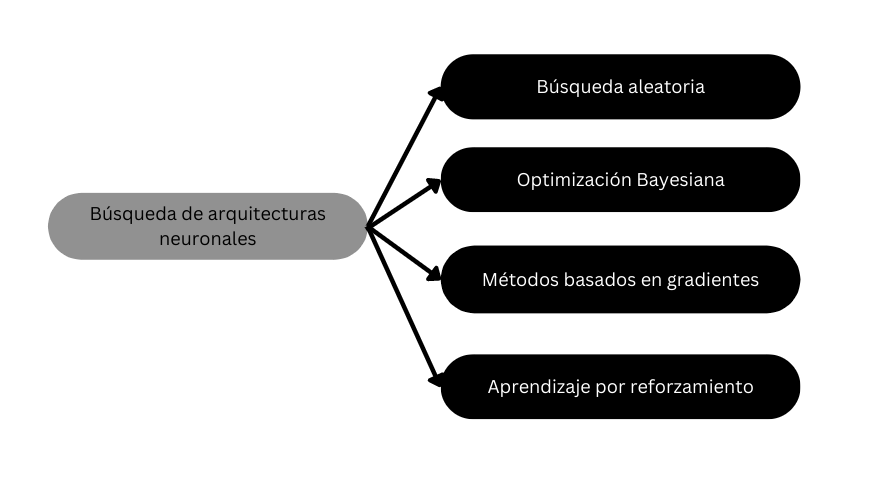
\includegraphics[scale=0.4]{images/NAS.png}
    \caption{Técnicas de arquitecturas de redes neuronales}
\end{figure}

\textit{Random search} es uno de los enfoques más ingenuos y simples para la búsqueda de arquitectura de red. Por ejemplo, \parencite{40} han presentado un enfoque para encontrar una buena arquitectura de red mediante la búsqueda aleatoria combinada con un conjunto bien entrenado de pesos compartidos. \parencite{41} propusieron nuevas líneas de base de búsqueda de arquitectura de red que se basan en la búsqueda aleatoria con parada anticipada para la optimización de hiperparámetros. Los resultados muestran que la búsqueda aleatoria junto con la parada anticipada logra resultados de búsqueda de arquitectura de red en el estado del arte en dos marcadores NAS estándar..

\textit{Reinforcement Learning} \parencite{42} es otro enfoque que se ha utilizado para encontrar la mejor arquitectura de red. \parencite{43} utilizaron una red neuronal recurrente (LSTM) con refuerzo para componer la arquitectura de la red neuronal. Más específicamente, la red neuronal recurrente se entrena a través de un algoritmo de búsqueda basado en gradiente llamado REINFORCE \parencite{44} para maximizar la precisión esperada de la arquitectura de la red neuronal generada. \parencite{45} introdujo un algoritmo de \textit{meta-modeling} llamado MetaQNN basado en el aprendizaje por refuerzo para generar automáticamente la arquitectura de la red neuronal convolucional para una nueva tarea. Las capas de la red neuronal convolucional son elegidas secuencialmente por un agente de aprendizaje que está entrenado usando \textit{Q-learning} con una técnica de exploración $\mathcal{E}$-\textit{greedy}. Simplemente, el agente explora un espacio de búsqueda finito de un conjunto de arquitecturas e iterativamente descubre diseños de arquitectura con un rendimiento mejorado en la nueva tarea a aprender.

\textit{Gradient-based optimization} es otra forma común para búsquedas de arquitecturas de redes neuronales. \parencite{46} propuso un enfoque basado en la relajación contínua de la arquitectura neuronal permitiendo usar descenso del gradiente para la búsqueda de la arquitectura. Los experimentos mostraron que este enfoque sobresale en encontrar arquitecturas convolucionales de alto rendimiento para la clasificación de imágenes en CIFAR-10, y en los conjuntos de datos de \textit{ImageNet}. \parencite{47} propuso un enfoque de optimización del descenso del gradiente para aprender la arquitectura de la red y parámetros simultáneamente. \parencite{48} usaron un enfoque basado en el gradiente para aprender arquitectura de redes. Los resultados experimentales en dos arquitecturas de redes diferentes: \textit{ResNet} y \textit{ResNeXt} mostraron que este enfoque recae en mejor precisión una reducción significativa en el número de parámetros. 

\textit{Bayesian optimization} basado en procesos \textit{Gaussian} ha sido usado por \parencite{49} y \parencite{50} para abordar el problema de búsqueda de arquitectura de redes neuronales. En adición, muchos trabajos se enfocaron en usar modelos basados en árboles como \textit{random forests} y \textit{tree Parzen estimators} \parencite{51} para efectivamente optimizar la arquitectura de red al igual que sus hiperparámetros \parencite{52} \parencite{53} \parencite{54}. La optimización Bayesiana  puede superar a algoritmos evolutivos en algunos problemas \parencite{55}

\subsection{Estrategia de rendimiento}
El objetivo de NAS es típicamente encontrar arquitecturas que puedan obtener alto rendimiento en la predicción de datos no vistos. La opción simple es ejecutar un entrenamiento estándar y la validación de la arquitectura en los datos, pero esto desafortunadamente es costoso computacionalmente y limita el número de arquitecturas que pueden ser exploradas. Investigaciones más recientes se enfocan en el desarrollo de métodos que reducen el costo de estas estimaciones de rendimiento. \\

El rendimiento puede ser estimado basado en \textit{lower fidelities} del actual rendimiento luego de un entrenamiento completo(también llamado \textit{proxy metrics}). Estas \textit{lower fidelities} incluyen menor tiempo de entrenamiento (\parencite{56} \parencite{57}), entrenar un sunconjunto de los datos \parencite{58}, en imágenes de baja resolución \parencite{59}, o con menos filtros por capa y menos celdas. Mientras estas aproximaciones \textit{low-fidelity} reducen el costo computacional, también introducen un sesgo en la estimación, ya que normalmente se subestima el rendimiento. Esto puede que no sea problemático siempre que la estrategia de búsqueda solo se base en clasificar diferentes arquitecturas y la clasificación relativa permanezca estable. Sin embargo, resultados recientes indican que esta clasificación relativa puede cambiar drásticamente cuando la diferencia entre las aproximaciones baratas y la evaluación “completa” es demasiado grande \parencite{57}, lo que aboga por un aumento gradual de las fidelidades \parencite{60} \parencite{61}.\\

Otra estrategia aplicada con éxito a las redes neuronales convolucionales (Convolutional Neural Networks, CNN) es compartir pesos entre diferentes modelos, lo que se conoce como compartición de parámetros o compartición de pesos \parencite{62}. Para NAS diferenciables con un gran modelo one-shot, la compartición de parámetros se logra naturalmente ya que las arquitecturas y los pesos se entrenan conjuntamente. Sin embargo, entrenar el modelo one-shot puede ser difícil ya que contiene todas las operaciones posibles. Para acelerar aún más el proceso de entrenamiento, \textit{single-path one-shot} fue propuesto \parencite{63} en el que solo se activa una operación entre un par de entrada y salida durante cada paso. Para NAS sin un modelo \textit{one-shot}, compartir pesos entre diferentes arquitecturas es más difícil pero no del todo imposible. Por ejemplo, dado que se sabe que algunos filtros convolucionales son extractores de características comunes, heredar pesos de arquitecturas anteriores es factible y razonable en las CNN \parencite{64}. 




\chapter{Propuesta: Autogoal Model Based}\label{chapter:proposal}

Como se mencionó en la introducción, AutoGoal es un \textit{framework} de \textit{auto machine learning} escrito en python capaz de resolver problemas en diferentes dominios mediante la construcción de pipelines que representan posibles soluciones a un problema dado. Usuarios no tan expertos pueden usar esta librería interactuando con un API de alto nivel a través de la clase \textbf{AutoML} la cual engloba las diferentes etapas del proceso de AutoML en una interfaz caja negra, además usuarios más expertos pueden interactuar con un API de bajo nivel para realizar sus experimentaciones ya sea cambiando los valores de los parámetros, métricas, tipos de datos, etc.

La propuesta de esta tesis es añadir modelos pre-entrenados en diferentes dominios al framework de AutoGoal, el objetivo es que estos modelos puedan formar parte del espacio de búsqueda de AutoGoal, de forma tal que puedan ser candidatos a soluciones, esto trae como ventajas que no haya que entrenar modelos desde cero, muchos modelos preentrenados resuelven populares tareas de clasificación de imágenes, traducción, clasificación de audios, resumen, etc; compitiendo con el estado del arte actual lo que puede traer buenos resultados en un menor tiempo que compitan con soluciones de AutoGoal.

En este capítulo se hace uso de varias herramientas de \textit{HuggingFace} para darle solución a esta problemática mediante la selección de algunos modelos pre-entrenados en diferentes dominios basándose en su popularidad, ya sea mayor cantidad de descargas. Estos modelos se integran a AutoGoal haciendo uso de la biblioteca \textit{Transformers}, la cual se utiliza para realizar todo el proceso, desde la descarga del modelo, preparación de datos y reentrenamiento (\textit{fine tuning}).

\section{BEiT para clasificación de imágenes}
En esta sección se propone la integración del modelo preentrenado BEiT como algoritmo al \textit{framework} AutoGoal. Se usó como fuente la plataforma \textit{HuggingFace} la cual ofrece una api con diferentes \textit{checkpoints} del modelo BEiT, en ese caso se eligió el checkpoint 'microsoft/beit-base-patch16-224-pt22k-ft22k'.

Descripción de 'microsoft/beit-base-patch16-224-pt22k-ft22k'\footnote[1]{\url{https://huggingface.co/microsoft/beit-base-patch16-224-pt22k-ft22k}}: Modelo BEiT preentrenado de manera autosupervisada en \textit{ImageNet-22k}, también llamado \textit{ImageNet-21k}, conjunto de datos que contiene 14 millones de imágenes y 21841 clases, las imágenes se encuentran a una resolución de 224x224 píxeles, tal modelo fue ajustado(\textit{fine tune}) en el mismo conjunto de datos a una resolución de 224x224 píxeles.

Mediante el método \texttt{ from\_pretrained } de  la clase \texttt{ BeitForImageClassification } se descarga el modelo con sus pesos y además es cacheado, este método recibe como primer parámetro el \textit{path} del \textit{checkpoint} que se va a descargar, el cual se menciona arriba. Como se le va a hacer \textit{fine-tuning} a este \textit{checkpoint} es necesario redefinir el vocabulario, por lo que se tiene que pasar dos diccionarios que representan las etiquetas del conjunto de datos que se van a utilizar para reentrenar BEiT con sus respectivos ids únicos, es decir cada etiqueta tiene un número único, y mediante estos dos diccionarios se puede saber el id conociendo la etiqueta y viceversa, además se debe pasar el argumento \texttt{ ignore\_mismatched\_sizes=True }, esto asegurará que la capa de salida, se deseche y se reemplace por una nueva capa de salida para la clasificación que será inicializada aleatoriamente e incluye un número personalizado de neuronas.

\begin{verbatim}
    self._model = BeitForImageClassification.from_pretrained(
      self.model_checkpoint,
      label2id=self._label2id,
      id2label=self._id2label,
      ignore_mismatched_sizes = True
    )
\end{verbatim}

Luego se hace uso de la clase \texttt{TrainingArguments} con el objetivo de generar una instancia que luego será pasada al \texttt{Trainer}, esta recibe como primer argumento el nombre que tomará nuestro \textit{checkpoint} y luego recibe una serie de parámetros que definen el proceso de reentrenamiento del modelo, aquí se detallan los parámetros que se usaron para instanciar esta clase:

\begin{verbatim}
    args = TrainingArguments(
        "BEiT-fine-tuned",
        evaluation_strategy = self._evaluation_strategy,
        save_strategy = self._save_strategy,
        learning_rate = self._learning_rate,
        per_device_train_batch_size = self._batch_size,
        per_device_eval_batch_size = self._batch_size,
        gradient_accumulation_steps = self._gradient_accumulation_steps,
        num_train_epochs = self._num_train_epochs,
        warmup_ratio = self._warmup_ratio,
        logging_steps = 10,
        load_best_model_at_end = True,
        metric_for_best_model = "accuracy"
    )
\end{verbatim}

\begin{itemize}
    \item \texttt{evaluation\_strategy}: recibe un \textit{string} con los siguientes valores: 'no', 'epoch' o 'steps', el valor por defecto es 'no', es decir que no realiza validaciones durante el entrenamiento, se usó 'epoch' para que en cada época del entrenamiento se valide.
    \item \texttt{save\_strategy}: recibe un \textit{string} con los siguientes valores: 'no', 'epoch' o 'steps', el valor por defecto es 'steps', se usó 'epoch', para que se guarde una copia del modelo cada vez que se alcanza una época en el entrenamiento.
    \item \texttt{learning\_rate} es el radio de aprendizaje para el optimizador \textit{AdamW}.
    \item \texttt{per\_device\_train\_batch\_size} tamaño del \textit{batch} que se usará en el entrenamiento, se le asignó 64.
    \item \texttt{per\_device\_eval\_batch\_size} tamaño del \textit{batch} que se usará en la evaluación, se le asignó 64.
    \item \texttt{gradient\_accumulation\_steps} es una técnica en la que se puede entrenar en tamaños de \textit{batch} más grandes de lo que la máquina normalmente podría guardar en memoria, se le asignó 4.
    \item \texttt{num\_train\_epochs} cantidad de épocas que tendrá el entrenamiento, toma valores enteros, en caso de que sea un valor con coma, entonces la última época la realizará en base al por ciento que representa la parte decimal.
    \item \texttt{warmup\_ratio} proporción del total de pasos de entrenamiento usados para un \textit{linear\_warmup} desde 0 hasta el \textit{learning\_rate}
    \item \texttt{load\_best\_model\_at\_end} a este parámetro se le asignó el valor \texttt{True} y lo que hace es cargar el mejor checkpoint de todas las épocas de entrenamiento basándose en la métrica. Importante que si este valor es verdadero entonces \texttt{evaluation\_strategy} y \texttt{save\_strategy} deben tener el mismo valor.
    \item \texttt{metric\_for\_best\_model} este parámetro se usa junto con \texttt{load\_best\_model\_at\_end} para definir la métrica que se usará para comparar los checkpoints en cada época, se le asignó la métrica \textit{accuracy}.
\end{itemize}

Luego para hacer el reentrenamiento del modelo se crea una instancia de la clase \texttt{Trainer} que recibe como primer parámetro el modelo en este caso sería la instancia que se obtiene al llamar \texttt{from\_pretrained()} en la clase \texttt{BeitForImageClassification}, y como segundo parámetro la instancia de la clase \texttt{TrainingArguments} que se creó arriba, entonces se llama al método \texttt{train} de esta, que se encarga de correr el re-entrenamiento, para instanciar la clase \texttt{Trainer} se le pasa los siguientes parámetros:

\begin{verbatim}
    Trainer(
        self._model,
        args,
        train_dataset = train_ds,
        eval_dataset = val_ds,
        compute_metrics = self._compute_metrics,
        data_collator = self._collate_fn,
    )
\end{verbatim}

\textit{train\_ds} y \textit{eval\_ds} corresponden a los conjuntos de datos para el entrenamiento y la validación durante el proceso de \textit{fine tuning}, hay dos \textit{features} claves para el reentrenamiento, estos son \texttt{pixel\_values} y \texttt{label}, que representan las imágenes como tensores de \texttt{torch} y las etiquetas de las imágenes respectivamente, estos conjuntos de datos tienen que ser \textit{Callable}, es decir tienen que implementar el método \texttt{\_\_getitem\_\_} y cuando este sea llamado debe retornar un diccionario con las llaves \textit{pixel\_values} y \textit{label}, las cuales tendrán como valor el elemento en la posición de las listas \textit{pixel\_values} y \textit{label} en la que fue llamada el método \texttt{\_\_getitem\_\_}, además esta debe implementar el método \texttt{\_\_len\_\_}, para resolver esto se creó una clase llamada \texttt{IterDataset} que implementa lo antes descrito. Importante que las imágenes tengan una resolución acorde a la que dicta el modelo, por ejemplo en este caso se requiere que sean de 224x224 píxeles.

\textit{data\_collator} este método se encarga de formar un \textit{batch} de elementos del conjunto de datos durante el proceso de \textit{fine tuning}, ya sea del conjunto de entrenamiento o del conjunto de validación. Este método también es llamado cuando se quieren hacer predicciones.

\textit{compute\_metrics}: recibe como parámetro una instancia de la clase \texttt{EvalPrediction} que contiene dos llaves claves, \texttt{predictions} y \texttt{label\_ids} ambos arreglos de \textit{numpy}, el primero contiene las predicciones que hizo el modelo y el segundo las etiquetas en caso de que fueran pasadas, y se utiliza la métrica de \textit{accuracy} para compararlos.

\subsection{BEiT como algoritmo de Autogoal}
Para englobar lo mencionado, se creó una clase \texttt{BEiTClassifier} la cual implementa el método \texttt{run}, método común entre todos los algoritmos de AutoGoal, el cual llama al método \texttt{run} de la clase \texttt{BEiTClassifierWrapper} que funciona como encapsulador de la anterior mencionada y además posee los métodos necesarios para llevar a cabo todas las etapas del algoritmo, ya sea descargar el modelo, reentrenarlo(\textit{fine tuning}) y evaluarlo.

El método \texttt{fit} de \texttt{BEiTClassifierWrapper}  recibe las imágenes y las etiquetas que serán usadas para reentrenar a \textit{BEiT}, las imágenes las recibe como una secuencia de tensores de torch(\texttt{Seq[Tensor3]}) y las etiquetas serían un vector de categorías(\texttt{VectorCategorical}). Dentro del método \texttt{fit} se descarga el modelo, se divide el conjunto de datos en entrenamiento y validación utilizando el método de \textit{sklearn} \texttt{train\_test\_split} y se instancian como \texttt{IterDataset}, y luego se procede a instanciar las configuraciones y a correr el entrenamiento.

Esta clase implementa también el método \texttt{predict} que recibe como argumento las imágenes como secuencia de tensores de \textit{torch} con las cuales luego se llama al método \texttt{predict} del modelo.

Para el re-entrenamiento de este modelo se utilizó la métrica 'accuracy' con la cual se comparan las predicciones con las etiquetas referencias para saber que tan efectivo está siendo el proceso de \textit{fine tuning}.

Hiperparámetros a optimizar por Autogoal:
\begin{itemize}
    \item \textit{hidden\_act} función de activación no lineal (función o cadena) en el \textit{encoder} y el \textit{pooler}, los posibles valores son: 'gelu', 'relu', y 'gelu\_new'.
    \item \textit{layer\_norm\_eps} El epsilon usado por las capas de normalización de capas, toma un valor en el intervalo contínuo [1e-12, 1e-10].
    \item \textit{warmup\_ratio} proporción del total de pasos de entrenamiento usados para un \textit{linear\_warmup} desde 0 hasta el \textit{learning\_rate}, toma un valor en el intervalo contínuo [0.05, 0.2].
\end{itemize}

\section{T5-small para resumen de documentos}
En esta sección se propone la integración del modelo preentrenado T5 como algoritmo al \textit{framework} AutoGoal. Se usó como fuente la plataforma \textit{HuggingFace} la cual ofrece una api con acceso a diferentes \textit{checkpoints} del modelo T5, en ese caso se eligió el checkpoint 't5-small'.

Con T5, se propone reformular todas las tareas de NLP(\textit{natural language preprocessing}) en un formato de texto a texto unificado donde la entrada y la salida son siempre cadenas de texto, en contraste con los modelos de estilo BERT que solo pueden generar una etiqueta de clase o un intervalo de la entrada. El marco de texto a texto nos permite usar el mismo modelo, función de pérdida e hiperparámetros en cualquier tarea de NLP, incluyendo traducción automática, resumen de documentos, respuesta a preguntas y tareas de clasificación (por ejemplo, análisis de sentimientos). Incluso podemos aplicar T5 a tareas de regresión entrenándolo para predecir la representación de cadena de un número en lugar del número en sí.

Mediante el método \texttt{ from\_pretrained } de la clase \texttt{ AutoModelForSeq2SeqLM } se descarga el modelo con sus pesos y además es cacheado, este método recibe como primer parámetro el \textit{path} del \textit{checkpoint} que se va a descargar, el cual se menciona arriba.

\begin{verbatim}
    self._model = AutoModelForSeq2SeqLM.from_pretrained(
          self.model_checkpoint
        ).to(self._device)
\end{verbatim}

Como se necesita hacer un preprocesamiento a los documentos y a los resúmenes, se hace uso del método \texttt{from\_pretrained} de la clase \texttt{ AutoTokenizer } el cual descarga un procesador de texto de acuerdo al modelo que se va a reentrenar.

Una vez descargado el \texttt{tokenizer} se pasan los datos por un método de preprocesamiento, este preprocesamiento se hace lo mismo a la hora de entrenar que a la hora de predecir, y en el último caso puede ser que no se envíen los resúmenes. Para tokenizar los documentos es necesario añadir el prefijo \texttt{"summarize: "} ya que el modelo \textit{t5-small} puede también ser usado para traducir y es necesita saber que tarea va a desarrollar. Se le pasan los datos al \textit{tokenizer} con el argumento \texttt{truncation=True} de forma tal que una entrada más larga de lo que puede manejar el modelo será truncada a la máxima longitud.

Luego se hace uso de la clase \texttt{Seq2SeqTrainingArguments}  con el objetivo de generar una instancia que luego será pasada al \texttt{Seq2SeqTrainer}, esta recibe como primer argumento el nombre que tomará el \textit{checkpoint} y luego recibe una serie de parámetros opcionales que definen el proceso de reentrenamiento del modelo, como la tarea es del tipo secuencia a secuencia, estas clases tienen como prefijo \texttt{Seq2Seq}, aquí se detallan los parámetros que se usan para instanciar esta clase:

\begin{verbatim}
    args = Seq2SeqTrainingArguments(
      "t5-small-finetuned",
      evaluation_strategy = self._evaluation_strategy,
      learning_rate = self._learning_rate,
      per_device_train_batch_size = self._batch_size,
      per_device_eval_batch_size = self._batch_size,
      weight_decay = self._weight_decay,
      save_total_limit = 3,
      num_train_epochs = self._num_train_epochs,
      predict_with_generate = True,
      fp16=(self._device == "cuda")
    )
\end{verbatim}

\begin{itemize}
    \item \texttt{evaluation\_strategy}: recibe un \textit{string} con los siguientes valores: 'no', 'epoch' o 'steps', el valor por defecto es 'no', es decir que no realiza validaciones durante el entrenamiento, se asignó 'epoch' a este parámetro para que en cada época del entrenamiento se valide.
    \item \texttt{learning\_rate} es el radio de aprendizaje para el optimizador \textit{AdamW}.
    \item \texttt{per\_device\_train\_batch\_size} tamaño del \textit{batch} que se usará en el entrenamiento, se le asignó 64.
    \item \texttt{per\_device\_eval\_batch\_size} tamaño del \textit{batch} que se usará en la evaluación, se le asignó 64.
    \item \texttt{num\_train\_epochs} cantidad de épocas que tendrá el entrenamiento, toma valores enteros, en caso de que sea un valor con coma, entonces la última época la realizará en base al por ciento que representa la parte decimal.
    \item \texttt{weight\_decay} el decaimiento del peso para aplicar (si no es cero) a todas las capas en el optimizador AdamW.
\end{itemize}

Luego para hacer el reentrenamiento del modelo se crea una instancia de la clase \texttt{Seq2SeqTrainer} que recibe como primer parámetro el modelo en este caso sería la instancia que se obtuvo al llamar \texttt{from\_pretrained()} en la clase \texttt{Seq2SeqTrainer}, y como segundo parámetro la instancia de la clase \texttt{Seq2SeqTrainingArguments} que se creó arriba y posee la personalización del proceso de entrenamiento, entonces se llama al método \texttt{train} de esta, que se encarga de correr el re-entrenamiento, para instanciar la clase \texttt{Seq2SeqTrainer} se le pasan los siguientes parámetros:

\begin{verbatim}
    self._trainer = Seq2SeqTrainer(
      self._model,
      args,
      train_dataset = train_ds,
      eval_dataset = val_ds,
      data_collator = data_collator,
      tokenizer = self._tokenizer,
      compute_metrics = self._compute_metrics
  )
\end{verbatim}

\textit{train\_ds} y \textit{val\_ds} corresponden a los conjuntos de datos para el entrenamiento y la validación durante el proceso de \textit{fine tuning}, hay dos \textit{features} claves para el reentrenamiento, estos son \texttt{input\_ids} y \texttt{labels}, que representan los documentos luego de ser procesados  y los resúmenes luego de ser procesados respectivamente, estos conjuntos de datos tienen que ser \textit{Callable}, es decir tienen que implementar el método \texttt{\_\_getitem\_\_} y cuando este sea llamado debe retornar un diccionario con las llaves \texttt{input\_ids} y \texttt{labels}, las cuales tendrán como valor el elemento en la posición de las listas \texttt{input\_ids} y \texttt{labels} en la que fue llamada el método \texttt{\_\_getitem\_\_}, además esta debe implementar el método \texttt{\_\_len\_\_}, para resolver esto se creó una clase llamada \texttt{IterDataset} que implementa lo antes descrito.

\textit{data\_collator} este método se encarga de formar un \textit{batch} de elementos del conjunto de datos durante el proceso de \textit{fine tuning}, ya sea del conjunto de entrenamiento o del conjunto de validación. Este método también es llamado cuando se quieren hacer predicciones.

\textit{compute\_metrics}: recibe como parámetro una instancia de la clase \texttt{EvalPrediction} que contiene dos llaves claves, \texttt{predictions} y \texttt{label\_ids} ambos arreglos de \textit{numpy}, el primero contiene las predicciones que hizo el modelo y el segundo las etiquetas en caso de que fueran pasadas, se hace un poco de preprocesamiento para descodificar y se utiliza la métrica de \textit{rouge} para comparar.

\subsection{T5-small como algoritmo de Autogoal}
Para englobar lo mencionado, se creó una clase \texttt{T5SmallSummarization} la cual implementa el método \texttt{run}, método común entre todos los algoritmos de AutoGoal, que llama al método \texttt{run} de la clase \texttt{T5SmallSummarizationWrapper} que funciona como encapsulador de la anterior mencionada y además posee los métodos necesarios para llevar a cabo todas las etapas del algoritmo, ya sea descargar el modelo, reentrenarlo(\textit{fine tuning}) y evaluarlo.

El método \texttt{fit} de \texttt{T5SmallSummarizationWrapper} recibe los documentos y los resúmenes que serán usadas para reentrenar a \textit{T5-small}, los documentos los recibe como una secuencia de documentos (\texttt{Seq[Document]}) y los resúmenes serían una secuencia de oraciones(\texttt{Seq[Sentence]}). Dentro del método \texttt{fit} se descarga el modelo y el tokenizador, se divide el conjunto de datos en entrenamiento y validación utilizando el método de \textit{sklearn} \texttt{train\_test\_split} y se instancian como \texttt{IterDataset}, y luego se procede a instanciar las configuraciones y a correr el entrenamiento.

Esta clase implementa también el método \texttt{predict} que recibe como argumento los documentos como una secuencia de documentos (\texttt{Seq[Document]}) con las cuales luego se llama al método \texttt{predict} del modelo.

Para el re-entrenamiento de este modelo se usó la métrica de ROUGE(\textit{Recall-Oriented Understudy for Gisting Evaluation}), es un conjunto de métricas que se utilizan para evaluar modelos que hacen resumen de documentos y traducción automática en el dominio de procesamiento del lenguaje natural.

Hiperparámetros a optimizar por Autogoal:
\begin{itemize}
    \item \textit{feed\_forward\_proj} Tipo de capa de avance a utilizar, los posibles valores son: 'relu' y 'gated-gelu'.
    \item \textit{weight\_decay} el decaimiento del peso para aplicar (si no es cero) a todas las capas en el optimizador AdamW.
\end{itemize}

\section{Requerimientos}
Es necesario tener instaladas las liberías \textit{transformers}(version 4.24.0), \textit{datasets}(version 2.7.1) y \textit{nltk} para el correcto funcionamiento de estos algoritmos.
\chapter{Detalles de Implementación y Experimentos}\label{chapter:implementation}
Para la experimentación de la integración de los dos algoritmos mencionados en el capítulo anterior solo se tuvo en cuenta que AutoGoal los detectara en dependencia de los tipos semánticos de la entrada y la salida de estos algoritmos, además de que llama al método \textit{fit} donde se realiza el re-entrenamiento de estos con una configuración de los hiperparámetros definidos. 

El algoritmo de clasificación de imágenes(BEiTClassifier) fue efecutado independientemente en Google Colab, con el dataset cifar10 y se obtuvieron los siguientes resultados.

\begin{verbatim}
***** Running training *****
  Num examples = 50000
  Num Epochs = 3
  Instantaneous batch size per device = 64
  Total train batch size (w. parallel, distributed & accumulation) = 256
  Gradient Accumulation steps = 4
  Total optimization steps = 585
  Number of trainable parameters = 85769674

Epoch  Training Loss  Validation Loss  Accuracy
0      0.336400       0.065284         0.980100
1      0.250400       0.044352         0.985600
2      0.224500       0.035686         0.989300
\end{verbatim}

En cuanto al algoritmo para realizar resúmenes de documentos(T5SmallSummarization) no se logró ejecutar completo para un dataset debido a que presenta muchos hiperparámetros y tarda mucho el re-entrenamiento de este.

Se logró integrar los modelos en AutoGoal los cuales se descubren automáticamente y se evaluó que eran compatibles con la arquitectura de autogoal y son descubiertos en dependencia de los tipos semánticos de la entrada y la salida. Debido al alto costo de la experimentación no fue posible hacer experimentos cuantitativos en donde se entrenaran estos algoritmos completos por lo que queda propuesto como trabajo futuro.


\backmatter

\begin{conclusions}
    Es de vital importancia seguir haciendo aportes al campo de AutoML con el objetivo de democratizar el uso de la inteligencia artificial, estos sistemas permiten encontrar soluciones factibles sin necesariamente ser expertos en el tema además de ahorrarnos tiempo de investigación y diseño.

    En esta tesis se implementó e integró dos modelos pre-entrenados como algoritmos a Autogoal, estos modelos fueron extraídos de la plataforma HuggingFace la cual provee una api que permite descargarlos, personalizar la configuración del re-entrenamiento y re-entrenarlos(\textit{fine tuning}). Específicamente estos modelos son \textit{checkpoints} de BEiT y de T5. 

    En la implementación para cada modelo se crearon dos clases, un wrapper que implementa los métodos para el re-entrenamiento y para la evaluación, y la clase principal que hereda de este wrapper y solo implementa el método run, se añadió un algoritmo para la clasificación de imágenes, y otro algoritmo para el resumen de documentos. Ambos algoritmos utilizan modelos pre-entrenados que fueron elegidos en cuanto a su popularidad en HuggingFace. A pesar de lograrse la integración de estos con AutoGoal y que sean detectados en el pipeline no se pudo experimentar mucho debido a la demanda de recursos y tiempo necesarios para re-entrenar estos algoritmos.
\end{conclusions}

\begin{recomendations}
    Los modelos pre-entrenados para ser adaptados a un problema en cuestión necesitan pasar por un proceso de re-entrenamiento(\textit{fine tuning}), para esto es necesario tener un conjunto de entrenamiento y uno de validación. El proceso de \textit{fine tuning} de los modelos que se añadieron como algoritmos a AutoGoal se realiza en el método \textit{fit}. Utilizando el método \textit{train\_test\_split} de \textit{Sklearn} se divide la entrada que recibe el algoritmo en un conjunto de entrenamiento y otro de validación. Algo que se puede mejorar es que para este tipo de algoritmos(algoritmos conformados por modelos pre-entrenados) exista forma de pasar estos dos conjuntos como entrada, ya que muchas veces los conjuntos vienen separados para este tipo de tareas(para el entrenamiento y la validación), de esta forma no se tomaría el propio conjunto de entrenamiento para validar también.

    Además debemos tener en cuenta que los modelos preentrenados poseen muchísimos parámetros por lo que re-entrenarlos requiere de muchos recursos y tiempo, es importante entonces que la cantidad de ejecuciones que haga AutoGoal sobre estos algoritmos para encontrar el mejor ajuste sea lo mínimo posible.
\end{recomendations}

\include{BackMatter/Bibliography}

\end{document}
